\documentclass[../DS02.tex]{subfiles}%
\graphicspath{{./figures/}}%

% \subimport{/home/nora/Documents/Enseignement/Prepa/bpep/exercices/DS/lentille_app_photo/}{sujet.tex}

\begin{document}%
\section[65]"P"{Guirlandes électriques}

\enonce{%
	Dans ce problème, on cherche à optimiser l'alimentation électrique d'un
	système comportant deux guirlande électriques $G_1$ et $G_2$,
	chacune étant modélisée par un conducteur ohmique de résistance
	identique $R_1 = R_2 = R$.

	La première guirlande est dédiée à un fonctionnement continu. La seconde
	est associée avec un interrupteur $S$ en série qui bascule de manière
	périodique afin de produire un clignotement.

	On supposera dans ce problème que la puissance lumineuse fournie par ces
	guirlandes est proportionnelle à la puissance électrique qu'elles
	reçoivent.
}%

\subsection{Système de base}

\enonce{%
	\noindent
	\begin{minipage}[c]{.65\linewidth}
		On considère dans un premier temps le circuit ci-contre alimenté par un
		générateur réel de f.e.m. $E$ et de résistance interne $r$.
		\textbf{Les expressions demandées ne feront intervenir que $E,r$ et
			$R$.}
		\smallbreak
		\emph{On considère que l'interrupteur $S$ est ouvert
			(Figure~\ref{fig:baseplain}).}
	\end{minipage}
	\hfill
	\begin{minipage}[c]{.30\linewidth}
		\begin{center}
			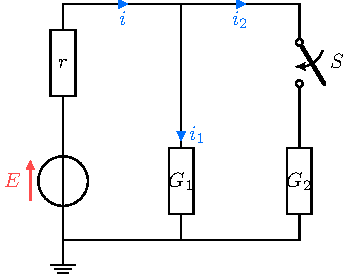
\includegraphics[width=\linewidth]{guirlande_base_plain}
			\captionof{figure}{}
			\label{fig:baseplain}
		\end{center}
	\end{minipage}
}%

\QR[2]{%
	Quelle est la puissance reçue $\Pc_{2,o}$ par la seconde
	guirlande $G_2$?
}{%
	L'intensité $i_2$ est alors nulle \pt{1}, donc $\boxed{\Pc_{2,o} = 0}$. \pt{1}
}%

\QR[6]{%
	Établir l'expression du courant $i_o$ passant à travers le générateur. En
	déduire que la puissance électrique $\Pc_{1,o}$ reçue par la guirlande $G_1$
	s'exprime~:
	\[
		\Pc_{1,o} = R \left( \frac{E}{r+R} \right)^2
	\]
}{%
	Le circuit est équivalent à~:
	\smallbreak
	\begin{isd}[lefthand ratio=.25]
		\begin{center}
			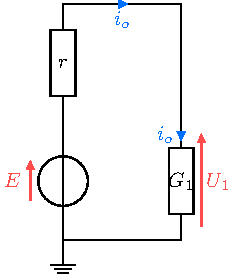
\includegraphics[scale=1]{guirlande_base_G1only}
			\captionof{figure}{\protect\pt{1}}
		\end{center}
		\tcblower
		La loi des mailles donne~:
		\[
			E \stm{=} i_0(r+R)
			\Ra
			\boxed{i_0 \stm{=} \frac{E}{r+R}}
		\]
		Or, d'après la loi d'\textsc{Ohm}, $U_1 = Ri_0$ \pt{1}.
		\smallbreak
		D'où la puissance reçue par $G_1$~:
		\[
			\boxed{\Pc_{1,o} \stm{=} i_o U_1 \stm{=} R \left( \frac{E}{r+R} \right)^2}
		\]
	\end{isd}
}%

\enonce{%
	\emph{On considère désormais que l'interrupteur $S$ est fermé.}
}%

\QR[5]{%
	Établir l'expression du courant $i_f$ passant à travers le
	générateur.
}{%
	Les deux guirlandes sont en dérivation.
	\smallbreak
	\begin{isd}[lefthand ratio=.25]
		\begin{center}
			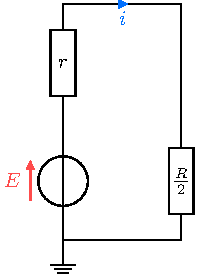
\includegraphics[scale=1]{guirlande_base_G1R2}
			\captionof{figure}{\protect\pt{1}}
		\end{center}
		\tcblower
		On peut les remplacer par une résistance équivalente~:
		\begin{gather*}
			\frac{1}{R\ind{eq}} \stm{=} \frac{1}{R} + \frac{1}{R}
			\Lra
			\boxed{R\ind{eq} \stm{=} \frac{R}{2}}
		\end{gather*}
		La loi des mailles donne~:
		\[
			E \stm{=} i_f \left( r + \frac{R}{2} \right)
			\Ra
			\boxed{i_f \stm{=} \frac{E}{r+\frac{R}{2}}}
		\]
	\end{isd}
}%

\QR[3]{%
	À l'aide d'un pont diviseur de courant, déterminer les expressions de
	$i_{1,f}$ et $i_{2,f}$.
}{%
	Pour $i_{k,f}$ découlant de $i_f$, avec $R\ind{eq}$ la résistance équivalente
	en parallèle et $R_k$ la résistance dans la branche, on a
	\begin{gather*}
		i_{k,f} \stm{=} \frac{R\ind{eq}}{R_k}i_f
		\qso
		i_{k,f} = \frac{R/2}{R}i_f
		\\\beforetext{d'où}
		\boxed{i_{1,f} \stm{=} \frac{E}{2r+R} = i_{2,f}}
	\end{gather*}
	\pt{1} pour un schéma.
}%

\QR[2]{%
	En déduire que les puissances $\Pc_{1,f}$ et $\Pc_{2,f}$ reçues par les deux
	guirlandes s'expriment~:
	\[
		\Pc_{1,f} = \Pc_{2,f} = R \left( \frac{E}{2r+R} \right)^2
	\]
}{%
	On a simplement
	\[
		\Pc_{k,f} \stm{=} R i_{k,f}
		\Ra
		\boxed{\Pc_{1,f} \stm{=} \Pc_{2,f} = R \left( \frac{E}{2r+R} \right)^2}
	\]
}%

\enonce{%
	\emph{Comparaisons des 2 situations.}
}%

\QR[3]{%
	La puissance reçue par la première guirlande est-elle identique dans les deux
	situations étudiées ($S$ ouvert et fermé)? Sachant qu'elle ne doit pas
	clignoter, est-ce un problème? Expliquer.
}{%
	On a~:
	\[
		\Pc_{1,o} = R \left( \frac{E}{r+R} \right)^2
		\stm{\neq}
		\Pc_{1,f} = R \left( \frac{E}{2r+R} \right)^2
	\]
	La guirlande 1 va donc se mettre à clignoter \pt{1}, puisque la puissance
	lumineuse qu'elle émet varie périodiquement. Ce montage ne \textbf{satisfait
		donc pas le cahier des charges}. \pt{1}
}%

\QR[3]{%
	Comment doit-on choisir $r$ par rapport à $R$ pour limiter le
	problème? Cette condition est-elle vérifiée pour
	$r = R = \SI{1}{\ohm}$?
}{%
	Pour limiter cet effet, il faut que $\boxed{r \ll R}$ \pt{1}. Dans ce cas, on
	peut négliger $r$ devant $R$, et il vient
	\[
		\boxed{
			\Pc_{1,o} \approx \Pc_{1,f} \stm{\approx} R \left( \frac{E}{R} \right)^2
		}
	\]
	Ce n'est pas le cas avec les valeurs données dans l'énoncé. \pt{1}
}%

\subsection{Système amélioré}

\enonce{%
	\noindent
	\begin{minipage}[c]{.65\linewidth}
		On considère maintenant le circuit ci-dessous afin de limiter la
		variation de puissance électrique reçue par la première guirlande, donc
		la variation du courant $i_1$.

		Une bobine d'inductance $L$ a donc été ajoutée en série avec la
		première guirlande. L'interrupteur $S$ est ouvert de manière
		périodique pour $t \in \left[0 ; \frac{T}{2} \right[$ et fermé pour
		$t \in \left[ \frac{T}{2} ; T\right[$.
	\end{minipage}
	\hfill
	\begin{minipage}[c]{.30\linewidth}
		\begin{center}
			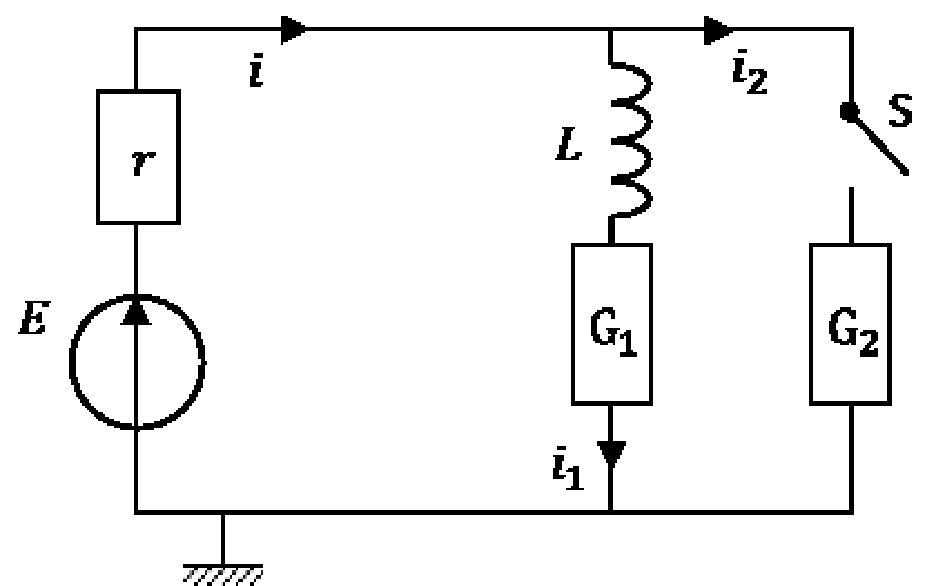
\includegraphics[width=\linewidth]{guirlande_better_plain}
			\captionof{figure}{}
			\label{fig:betterplain}
		\end{center}
	\end{minipage}
}%

\QR[2]{\label{q:pcont}%
	En régime stationnaire (permanent continu), donner le schéma équivalent du
	nouveau montage.
}{\label{q:pcont}%
	En régime stationnaire, la bobine est équivalente à un fil électrique \pt{1}.
	Le montage est donc équivalent à celui de la partie précédente. \pt{1}
}%

\enonce{%
	\emph{On se place juste avant la fermeture de l'interrupteur},
	c'est-à-dire en $t = \frac{T}{2}^-$, et on admet que le régime
	stationnaire a été atteint.
}%

\QR[3]{%
	Déterminer la valeur de $i_1\left(\frac{T}{2}^-\right)$. En déduire
	la valeur de $i_1\left(\frac{T}{2}^+\right)$.
}{%
	Puisque le montge est équivalent à celui de la partie précédente, on sait
	que~:
	\[
		i_1 \left( \frac{T}{2}^- \right) \stm{=} \frac{E}{r+R}
	\]
	Or, le courant traversant une bobine est continu \pt{1}, soit
	\[
		i_1 \left( \frac{T}{2}^- \right) =
		i_1 \left( \frac{T}{2}^+ \right) \stm{=}
		\frac{E}{r+R}
	\]
}%

\QR[5]{\label{q:beforeT2}%
	Déterminer les valeurs de $i_2\left(\frac{T}{2}^-\right)$ et
	$i_2\left(\frac{T}{2}^+\right)$.
}{\label{q:beforeT2}%
	L'interrupteur étant ouvert, on a~:
	\[
		\boxed{i_2 \left( \frac{T}{2}^- \right) \stm{=} 0}
	\]
	Une fois l'interrupteur fermé, la loi des mailles à $t = \frac{T}{2}^+$
	donne~:
	\begin{DispWithArrows*}[]
		E &\stm{=} ri + Ri_2\left(\frac{T}{2}^+\right)
		\Arrow{$i \stm{=} i_1+i_2$}
		\\\Lra
		E &=
		r \left(
		i_1 \left(\frac{T}{2}^+\right) +
		i_2 \left(\frac{T}{2}^+\right)
		\right) +
		R i_2 \left(\frac{T}{2}^+\right)
		\Arrow{On isole}
		\\\Lra
		i_2 \left(\frac{T}{2}^+\right) &\stm{=}
		\frac{E - ri_1 (\frac{T}{2}^+)}{r+R}
		\Arrow{On remplace}
		\\\Lra
		i_2 \left(\frac{T}{2}^+\right) &=
		\frac{E - r \left( \frac{E}{r+R} \right)}{r+R}
		\Arrow{On simplifie}
		\\\Lra
		\Aboxed{i_2 \left(\frac{T}{2}^+\right) &\stm{=} E \frac{R}{(r+R)^2}}
	\end{DispWithArrows*}
}%

\enonce{%
\emph{On considère l'intervalle $\left[0 ; \frac{T}{2} \right[$,
lorsque l'interrupteur est ouvert.}
}%

\QR[5]{%
Établir l'équation différentielle dont $i_1$ est solution sur
l'intervalle $\left[0 ; \frac{T}{2} \right[$. On fera apparaître un
temps caractéristique $\tau_o$ en fonction de $L$, $r$ et $R$.
}{%
\smallbreak
\vspace{-25pt}
\begin{isd}[lefthand ratio=.35, interior hidden]
	\begin{center}
		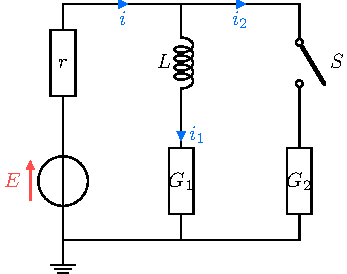
\includegraphics[scale=1]{guirlande_better_open}
		\captionof{figure}{\protect\pt{1}}
	\end{center}
	\tcblower
	Loi des mailles~:
	\begin{DispWithArrows*}[fleqn, mathindent=5pt]
		E &\stm{=} r_1i + u_L + Ri_1
		\Arrow{$u_L \stm{=} L \dv{i_1}{t}$}
		\\\Lra
		L \dv{i_1}{t} + (r+R)i_1 &= E
		\Arrow{Canonique}
		\\\Lra
		\Aboxed{\dv{i_1}{t} + \frac{i_1(t)}{\tau_o} &\stm{=} \frac{E}{L}}
		\qav
		\boxed{\tau_o \stm{=} \frac{L}{r+R}}
	\end{DispWithArrows*}
\end{isd}
}%

\enonce{%
\emph{On s'intéresse maintenant à l'intervalle
$\left[ \frac{T}{2} ; T\right[$, lorsque l'interrupteur est fermé.}
}%

\QR[8]{%
	Montrer que $i_1$ est solution de l'équation différentielle
	suivante~:
	\[\dv{i_1}{t} + \dfrac{i_1}{\tau_f} =
		\dfrac{E}{L\left(1 + \dfrac{r}{R}\right)}
		\qav
		\tau_f = \dfrac{L\left(1 + \dfrac{r}{R}\right)}{2r + R}
	\]
}{%
	\smallbreak
	\vspace{-25pt}
	\begin{isd}[lefthand ratio=.3, interior hidden]
		\begin{center}
			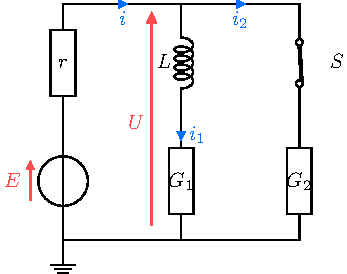
\includegraphics[scale=1]{guirlande_better_closed}
			\captionof{figure}{\protect\pt{1}}
		\end{center}
		\tcblower
		Loi des mailles et loi des nœuds~:
		\begin{DispWithArrows*}
			E &\stm{=} r_1i + Ri_1 + L \dv{i_1}{t}
			\Arrow{$i \stm{=} i_1+i_2$}
			\\\Lra
			E &= r (i_1+i_2) + Ri_1 + L \dv{i_1}{t}
		\end{DispWithArrows*}
		Or, avec les branches en parallèle,
		\[
			Ri_2 \stm{=} Ri_1 + L \dv{i_1}{t}
			\Ra
			i_2 \stm{=} i_1 + \frac{L}{R}\dv{i_1}{t}
		\]
	\end{isd}
	D'où en combinant~:
	\begin{DispWithArrows*}[]
		E &\stm{=}
		r \left( i_1 + i_1 + \frac{L}{R}\dv{i_1}{t} \right) + Ri_1 + L \dv{i_1}{t}
		\Arrow{On simplifie}
		\\\Lra
		E &= i_1 (2r+R) + L \left( 1 + \frac{r}{R} \right)\dv{i_1}{t}
		\Arrow{Canonique}
		\\\Lra
		\Aboxed{
			\dv{i_1}{t} + \frac{i_1(t)}{\tau_f} &\stm{=}
			\frac{E}{L \left(1 + \frac{r}{R}\right)}
		}
		\qav
		\boxed{\tau_f \stm{=} \frac{L \left( 1 + \frac{r}{R} \right)}{2r + R}}
	\end{DispWithArrows*}
}%

\QR[7]{%
	Donner la forme générale $i_1(t)$ de la solution de cette équation
	différentielle. On ne cherchera pas à déterminer la constante
	intervenant dans la solution.
}{%
	La solution générale est la somme de la solution homogène et de la solution
	particulière \pt{1}. Or, pour la solution homogène, en injectant $i_{1,h}(t) =
		A \exr^{rt}$ \pt{1} on obtient~:
	\[
		r + \frac{1}{\tau_f} = 0
		\Lra
		\boxed{r \stm{=} -\frac{1}{\tau_f}}
		\qso
		i_{1,h}(t) \stm{=} A \exr^{-\frac{t}{\tau_f}}
	\]
	De plus, avec $i_{1,p}$ la solution particulière constante, on trouve
	\begin{gather*}
		\frac{i_{1,p}}{\tau_f} = \frac{E}{L \left( 1+\frac{r}{R} \right)}
		\Lra
		i_{1,p} \stm{=}
		E \frac{
			\cancel{L} \bcancel{\left( 1+\frac{r}{R} \right)}
		}{%
			(2r+R) \cancel{L} \bcancel{\left( 1+\frac{r}{R} \right)}
		}%
		\\\Lra
		\boxed{i_{1,p} \stm{=} \frac{E}{2r+R}}
		\\\beforetext{Ainsi,}
		\boxed{i_1(t) \stm{=} A \exr^{-\frac{t}{\tau_f}} + \frac{E}{2r+R}}
	\end{gather*}
}%

\enonce{%
	On étudie expérimentalement les variations du courant $i_1(t)$ en mesurant la
	tension aux bornes de la guirlande $G_1$ à l'aide d'un
	oscilloscope et on obtient le résultat suivant (Figure~\ref{fig:itplain}) pour
	deux valeurs différentes de l'inductance $L$. La résistance $R$ vaut
	$\SI{2}{\ohm}$ et la résistance $r$ vaut $\SI{1}{\ohm}$.
	\begin{center}
		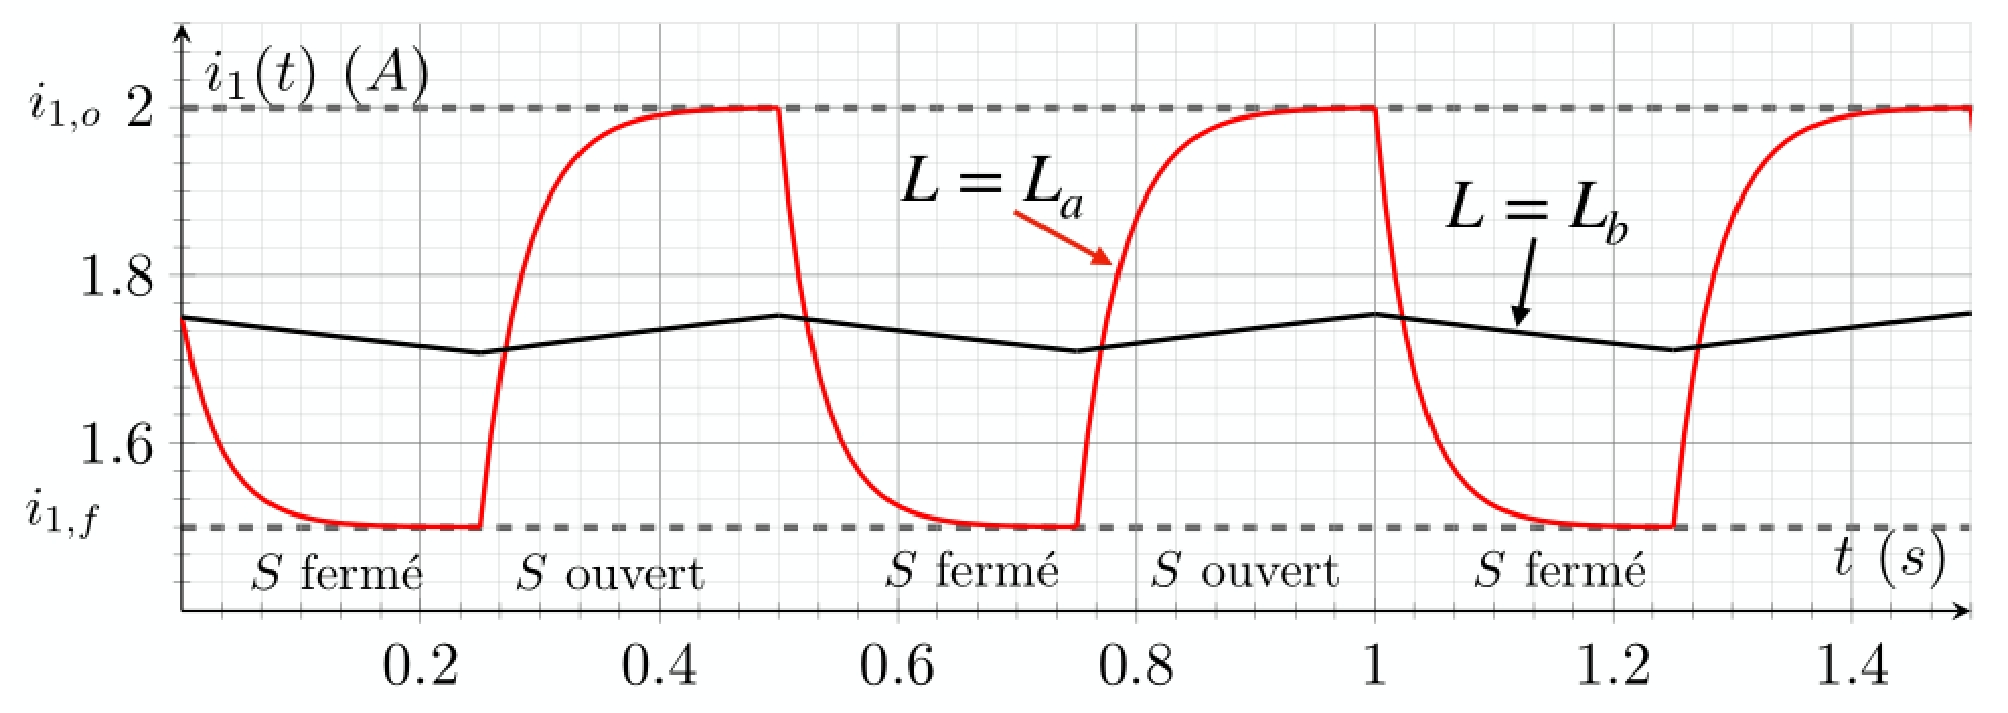
\includegraphics[width=.8\linewidth]{it_plain}
		\captionof{figure}{}
		\label{fig:itplain}
	\end{center}
}%

\QR[2]{%
	Parmi les deux bobines d'inductance $L_a$ et $L_b$, laquelle permet
	d'atteindre le régime stationnaire mentionné dans les questions
	\ref{q:pcont} à \ref{q:beforeT2}~?
}{%
	Il s'agit de la bobine $L_a$ \pt{1}, puisque la charge de la bobine a le temps
	de se faire entièrement. \pt{1}
}%

\QR[5]{%
	Retrouver, par lecture graphique, la valeur de $L_a$. Reproduire sommairement
	sur votre copie la Figure~\ref{fig:it_plain} et indiquer la construction à
	effectuer.
}{%
	Le temps $\tau_f$ correspond au temps nécessaire pour réaliser 63\% de la
	décharge de la bobine \pt{1}. À partir du point de bascule en $t = \SI{1}{s}$,
	63\% de la décharge correspond à une intensité de $\SI{1.69}{A}$, ce qui
	s'atteint pour $t_1 = \SI{1.033}{s}$~; ainsi,
	\begin{gather*}
		\xul{\tau_f = \SI{33}{ms}} \pt{1}
		\qet
		L_a \stm{=} \tau_f \frac{2r+R}{1+\frac{r}{R}}
		\qav
		\left\{
		\begin{array}{rcl}
			r & = & \SI{1}{\ohm}
			\\
			R & = & \SI{2}{\ohm}
		\end{array}
		\right.
		\quad
		\AN \xul{
			L_a \stm{=} \SI{88}{mH}
		}
	\end{gather*}
	\begin{center}
		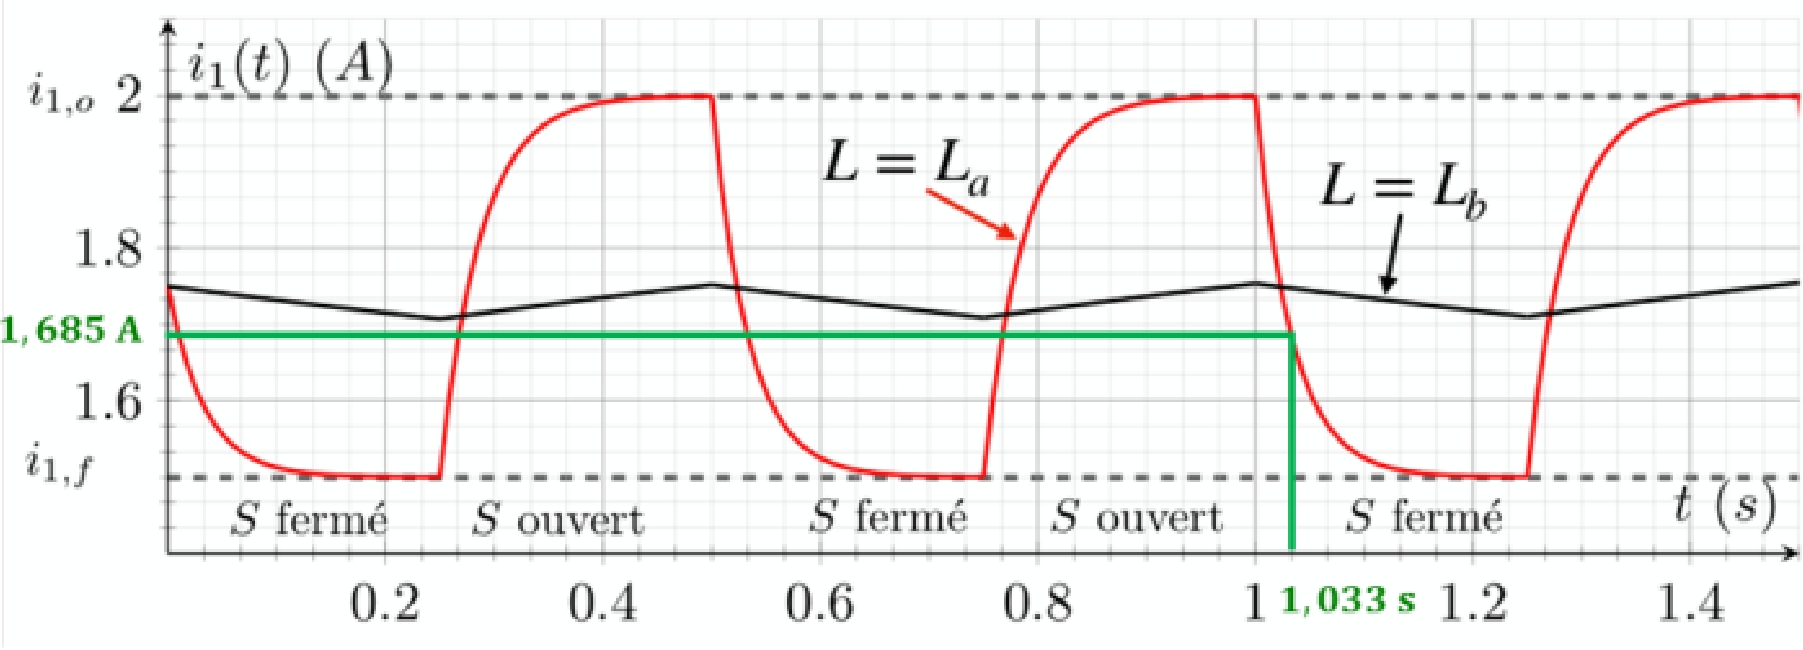
\includegraphics[width=.5\linewidth]{it_corr}
		\captionof{figure}{\protect\pt{1}}
		\label{fig:itcorr}
	\end{center}
	On peut également réaliser une tangente au point de bascule, et trouver
	l'intersection avec l'asymptote $i_1(t) = i_{1,f}$.
}%

\QR[2]{%
	Justifiez que $L_b \gg L_a$, sans chercher à déterminer sa valeur.
}{%
	Le temps caractéristique du régime transitoire avec $L_b$ est très supérieur
	devant celui avec $L_a$ \pt{1}, d'où $\boxed{L_b \gg L_a}$. \pt{1}
}%

\QR[2]{%
	Quelle est la valeur de l'inductance à retenir parmi $L_a$ et $L_b$ pour
	minimiser les variations de puissance reçue par la première guirlande?
}{%
	Il s'agit de $L_b$, \pt{1} car l'intensité $i_1(t)$ ne varie presque pas
	\pt{1} (et il en va de même pous la tension $U$).
}%

\end{document}%
